\documentclass[11pt]{article}
\usepackage[top=1cm, bottom=2cm, left=1cm, right=1cm]{geometry}
\usepackage{ctex}
\usepackage{algorithm}
\usepackage{algorithmicx}
\usepackage{algpseudocode}
\usepackage{amsthm,amsmath,amssymb}
\usepackage[colorlinks=true,linkcolor=blue]{hyperref}
\usepackage{listings}
\usepackage{xcolor,xparse}
\usepackage{realboxes}
\usepackage{graphics}
\usepackage{graphicx}
\usepackage{mathrsfs}
\usepackage{wrapfig}
\usepackage{subfigure}
\usepackage{pifont}
\newcommand{\To}{\textbf{To} }
\definecolor{cmdbg}{rgb}{0.9,0.9,0.9}
\lstset{%
	basicstyle=\ttfamily,
	breaklines = true,
	backgroundcolor=\color{cmdbg},
}
\DeclareDocumentCommand{\ccmd}{v}{% 参数 v 表示工作方法类似于 \verb
    \Colorbox{cmdbg}{\csname lstinline\endcsname!#1!}%
}

\makeatletter
\newenvironment{breakablealgorithm}
  {% \begin{breakablealgorithm}
   \begin{center}
     \refstepcounter{algorithm}% New algorithm
     \hrule height.8pt depth0pt \kern2pt% \@fs@pre for \@fs@ruled
     \renewcommand{\caption}[2][\relax]{% Make a new \caption
       {\raggedright\textbf{\ALG@name~\thealgorithm} ##2\par}%
       \ifx\relax##1\relax % #1 is \relax
         \addcontentsline{loa}{algorithm}{\protect\numberline{\thealgorithm}##2}%
       \else % #1 is not \relax
         \addcontentsline{loa}{algorithm}{\protect\numberline{\thealgorithm}##1}%
       \fi
       \kern2pt\hrule\kern2pt
     }
  }{% \end{breakablealgorithm}
     \kern2pt\hrule\relax% \@fs@post for \@fs@ruled
   \end{center}
  }
\makeatother

\author{谢昀城 22307110070}
\title{计算物理作业9}

\begin{document}
\maketitle




  \section{题目1}
  \subsection{题目描述}
  
  The interior of a 𝑑-dimensional hypersphere of unit radius is defined by the condition 
  . Write a program that finds the volume of a hypersphere using a Monte Carlo method. Test your program for $d=2$ and $d=3$ and then calculate the volume for $d=4$ and $d=5$, compare your results with the exact results.
\subsection{程序描述}
   在本程序中,我们使用蒙特卡洛方法计算d维超球体的体积,并计算了1-7维的体积,并比较了其与标准值的相对误差。其中程序使用线性同余算法生成均匀分布的伪随机数。

本程序源文件为sphere.py,在终端进入当前目录,使用命令python -u sphere.py运行本程序。运行时请保证Python第三方库Numpy,Matplotlib已安装。程序开发环境为Python3.12.3,可在Python3.8以上版本中运行。

\subsection{伪代码}
\subsubsection*{伪随机数生成 伪代码:}
\begin{breakablealgorithm}
  \caption{PRN}
  \begin{algorithmic}
    \Function{PRN}{$n,dim,rmin,rmax,seed$}
      \State \textbf{INPUT:} $n$ (number of rows), $dim$ (number of columns), $rmin$ (minimum range), $rmax$ (maximum range), $seed$ (initial seed)
      \State \textbf{OUTPUT:} $result$ (2D array of pseudo-random numbers)
      
      \State $m \gets 2^{31} - 1$,$a \gets 48271$,$b \gets 43$,$x \gets seed$
      \State $result \gets$ [] \Comment{Initialize empty list to store results}
      
      \For{$i \gets 0$ \To $n \cdot dim - 1$}
          \State $x \gets (a \cdot x + b) \% m$
          \State Append $rmin + (rmax - rmin) \cdot x / m$ to $result$
      \EndFor
  
      \State $result \gets$ Reshape(result, $n$, $dim$) \Comment{Convert the list to a 2D array}
      \State \Return $result$
    \EndFunction
  \end{algorithmic}
  \end{breakablealgorithm}
  
  \subsubsection*{蒙特卡洛积分伪代码}
  \begin{breakablealgorithm}
    \caption{intMcN}
    \begin{algorithmic}
      \Function{intMcN}{$fn,r,point$}
        \State \textbf{INPUT:} $fn$ (function to integrate), $r$ (function to rescale), $point$ (sampling points)
        \State \textbf{OUTPUT:} $result$ (Monte Carlo integral value)
        
        \State $result \gets$ Mean\Big([$fn(p)/r(p)$ for $p$ in $point$]\Big) \Comment{Compute average over sampling points}
        
        \State \Return $result$
      \EndFunction
    \end{algorithmic}
    \end{breakablealgorithm}
    
  
  
  
  \subsection{输入输出实例}

  对于本程序,运行后会生成图\ref{fig:prn}和图\ref{fig:v}为"PRN"和"VolumeDim.png"于当前目录下,分别为伪随机数采样和体积计算结果和相对误差,并在控制台打印计算结果。程序运行截图如图\ref{fig:p1}所示。可以看到,随着维数增加,计算结果的偏差也增加,这是由于高维空间的球体积占总采样体积的比例更小,采样更困难。
  \begin{figure}[ht]
    \centering
    \includegraphics[width=0.8\linewidth]{photo/PRN}
    \caption{PRN 采样分布(a)dimension=1(b)dimension=2}
    \label{fig:prn}
  \end{figure}

  \begin{figure}[ht]
    \centering
    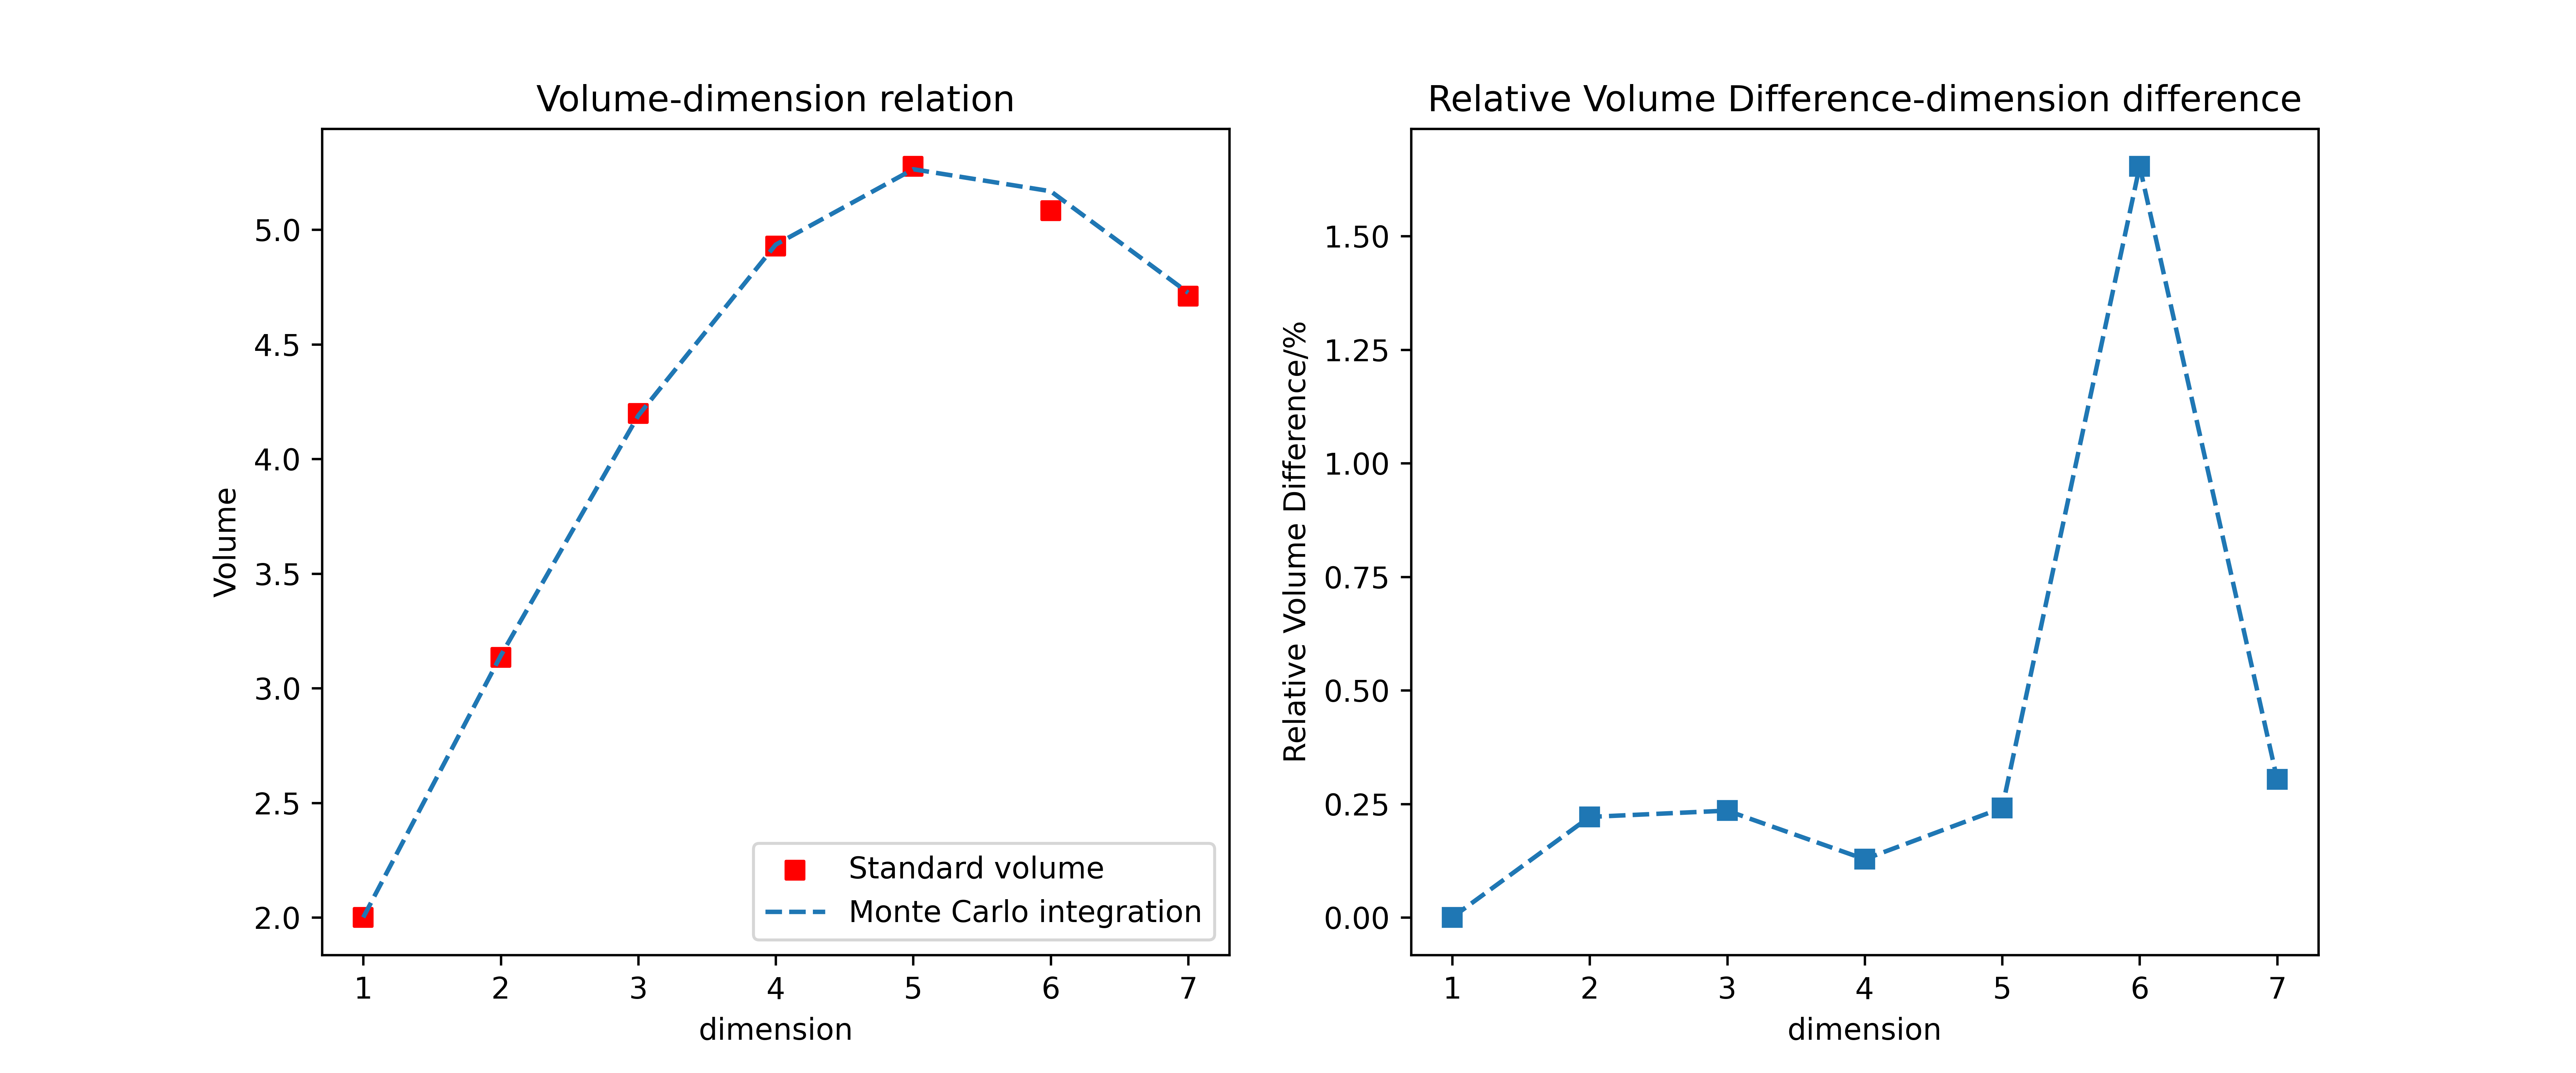
\includegraphics[width=1.0\linewidth]{photo/VolumeDim.png}
    \caption{(a)不同维度下球体积计算结果(b)与标准值相对误差}
    \label{fig:v}
  \end{figure}

  \begin{figure}
    \centering
    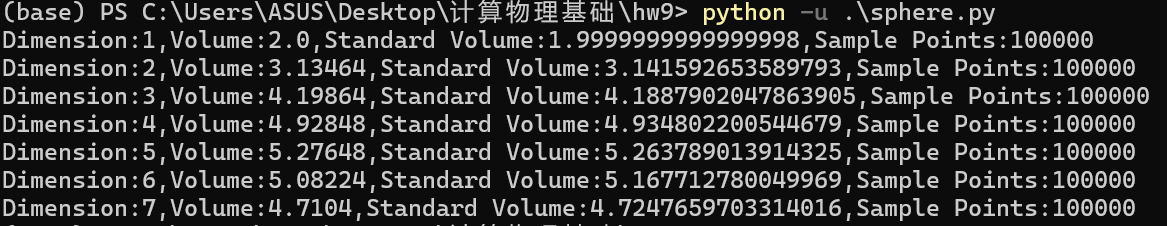
\includegraphics[width=0.6\linewidth]{photo/figp1.png}
    \caption{题目1程序运行截图}
    \label{fig:p1}
  \end{figure}

  \section{题目2}

  Write a MC code for a 3D Face-Centered Cubic lattice using the Heisenberg spin
model (adopt periodic boundary condition). Estimate the ferromagnetic Curie temperature.
\[
    H = -J \sum_{\langle i,j \rangle} \vec{S}_i \cdot \vec{S}_j, \quad J = 1, \quad |\vec{S}_i| = 1
\]

\subsection{程序描述}
本程序中,我们通过metropolis算法求解三维fcc晶格上的海森堡模型,主要求解功能在Heisenberg类中实现。程序将计算并可视化$4\times 4\times 4$个初基元胞上,$\frac{k_B T}{J}=1.0,6.0$时的平衡构型。并在不同尺寸下($L\times L\times L,L=2,3,4,5$)求解$<E>$,$<M>$,$<C>$,$<\chi>$随温度变化的关系,以得到相变温度。

其中,热容$C$和磁化率$\chi$将通过采样系统能量和磁矩的涨落得到:
\[
    C = \frac{<E^2>-<E>^2}{N k_B T^2},\quad \chi = \frac{<M^2>-<M>^2}{N k_B T}
\]
程序将首先使用$1000 L^3$个MC步进行热平衡,然后在平衡构型下运行$2000 L^3$个MC步,每$L^3$步采样体系的能量和平均磁矩。为了避免磁畴产生而难以达到平衡,系统将从$\vec{S_i}=(1,0,0)$的基态构型开始。

由于系统尺寸$L \to \infty$时,$\chi$将在$T_c$处发散,因此我们将取$\chi$最大时的温度作为体系相变温度。

本程序将使用Marsaglia算法生成球面上的均匀分布。

本程序源文件为Heisenberg.py,在终端进入当前目录,使用命令python -u Heisenberg.py运行本程序。运行时请保证Python第三方库Numpy,Numba,Matplotlib已安装。程序开发环境为Python3.12.3,可在Python3.8以上版本中运行。


\subsection{伪代码}
\subsubsection*{Marsaglia算法生成球面均匀分布}
\begin{breakablealgorithm}
  \caption{Marsaglia}
  \begin{algorithmic}
    \Function{Marsaglia}{}
      \State \textbf{INPUT:} None
      \State \textbf{OUTPUT:} $result$ (array of three numbers generated using Marsaglia method)
  
      \While{True}
          \State $v1 \gets 2 \cdot$ Random() $- 1$
          \State $v2 \gets 2 \cdot$ Random() $- 1$
          \State $s \gets v1^2 + v2^2$
          \State $s2 \gets \sqrt{1 - s}$
          \If{$s < 1$}
              \State \Return $\text{Array}([2 \cdot v1 \cdot s2, 2 \cdot v2 \cdot s2, 1 - 2 \cdot s])$
          \EndIf
      \EndWhile
    \EndFunction
  \end{algorithmic}
  \end{breakablealgorithm}
  \subsubsection*{求解Heisenberg模型}
  \begin{breakablealgorithm}
    \caption{Heisenberg Class}
    \begin{algorithmic}
    \State \textbf{Class: Heisenberg}
        \State \textbf{Attributes:}
            \State $L$: Lattice size (integer)
            \State $T$: Temperature (float)
            \State $J$: Interaction constant (default = $-1.0$)
            \State $baiss$: Array defining lattice basis
            \State $lattice$: FCC lattice positions
            \State $spins$: Spin vectors at lattice sites
            \State $neighbors$: List of neighbor indices for each lattice site
        
        \State \textbf{Methods:}
    
        \Function{Init}{$L$, $T$, $J = -1.0$}
            \State $self.L \gets L$, $self.T \gets T$, $self.J \gets J$
            \State $self.baiss \gets \text{Array}([[0, 0, 0], [0, 0.5, 0.5], [0.5, 0, 0.5], [0.5, 0.5, 0]])$
            \State \Call{GenerateFCCLattice}{}
            \State \Call{SetSpins}{}
            \State \Call{InitializeNeighbors}{}
        \EndFunction
    
        \Function{GenerateFCCLattice}{}
            \State $lattice \gets \text{Empty List}$
            \For{$i \gets 0$ to $L - 1$}
                \For{$j \gets 0$ to $L - 1$}
                    \For{$k \gets 0$ to $L - 1$}
                        \For{$b$ in $self.baiss$}
                            \State Append $[i, j, k] + b$ to $lattice$
                        \EndFor
                    \EndFor
                \EndFor
            \EndFor
            \State $self.lattice \gets \text{Array}(lattice)$
        \EndFunction
    
        \Function{InitializeNeighbors}{}
            \State $neighbors \gets \text{Empty List}$
            \State $nbDistance \gets \text{Array}([[0, 0.5, 0.5], [0.5, 0, 0.5], [0.5, 0.5, 0]])$,$tol \gets 10^{-5}$
            \For{$i, r_i$ in $\text{Enumerate}(self.lattice)$}
                \State $neighbor \gets \text{Empty List}$
                \For{$j, r_j$ in $\text{Enumerate}(self.lattice)$}
                    \State $r_{ij} \gets r_i - r_j$
                    \State \Call{ApplyPBC}{$r_{ij}$}
                    \If{$i \neq j$ \textbf{and} $abs(r_{ij})$ is close to any $nbDistance$ within $tol$}
                        \State Append $j$ to $neighbor$
                    \EndIf
                \EndFor
                \State Append $neighbor$ to $neighbors$
            \EndFor
            \State $self.neighbors \gets \text{Array}(neighbors)$
        \EndFunction
    
        \Function{ApplyPBC}{$r_{ij}$}
            \For{$i \gets 0$ to $2$}
                \If{$r_{ij}[i] > L / 2$}
                    \State $r_{ij}[i] \gets r_{ij}[i] - L$
                \ElsIf{$r_{ij}[i] < -L / 2$}
                    \State $r_{ij}[i] \gets r_{ij}[i] + L$
                \EndIf
            \EndFor
        \EndFunction
    
        \Function{CalculateEnergy}{}
            \State $s_n \gets \text{self.spins[self.neighbors]}$
            \State \Return $J \cdot \text{Sum}(\text{self.spins[:, None, :]} \cdot s_n) / 2 / \text{Length(self.lattice)}$
        \EndFunction
    
        \Function{CalculateMagnetization}{}
            \State \Return $\text{Sum}(self.spins, \text{axis} = 0) / \text{Length}(self.lattice)$
        \EndFunction
    
        \Function{CalculateDeltaE}{$i, spin1, spin2$}
            \State $dS \gets spin2 - spin1$
            \State $dE \gets J \cdot \text{Sum}(dS \cdot \text{self.spins[self.neighbors[i]]})$
            \State \Return $dE$
        \EndFunction
    
        \Function{MetropolisStep}{}
            \State $index \gets \text{Random Integer in Range}(\text{Length}(self.spins))$
            \State $spin1 \gets self.spins[index]$
            \State $spin2 \gets \text{Marsaglia()}$
            \State $dE \gets \Call{CalculateDeltaE}{index, spin1, spin2}$
            \If{$dE < 0$ \textbf{or} $\text{Random()} < \exp(-dE / T)$}
                \State $self.spins[index] \gets spin2$
            \EndIf
        \EndFunction
    \end{algorithmic}
    \end{breakablealgorithm}
    
\subsection{输入输出实例}
对于本程序,运行后会生成图\ref{fig:mar},\ref{fig:t1},\ref{fig:t6},\ref{fig:Tc}为"Marsaglia.png","T=1.0.png","T=6.0.png","fingTc.png"于当前目录下,分别为球面随机向量的生成,T=1.0,6.0时的平衡结构,不同$L$,$<E>,<|M|>,C,\chi$随$T$的变化。程序运行截图如图\ref{fig:p2}所示。

可以看到,在低温时,磁矩朝向几乎一致(图\ref{fig:t1}),高温时则呈现混乱分布(图\ref{fig:t6})。

随着温度的升高,$<|M|>$在$T_c$附近下降到0,$<E>$随温度的增加速率减慢。而$C$和$\chi$在$T_c$附近有明显的峰值,且随着系统尺寸$L$的增加,峰值宽度减小,峰值增加,表现出明显的有限尺寸效应(图\ref{fig:Tc})。

最终得到相变温度约为:
\[T_c\approx 3.19 \frac{J}{k_B}\]

\begin{figure}[htpb]
    \centering
    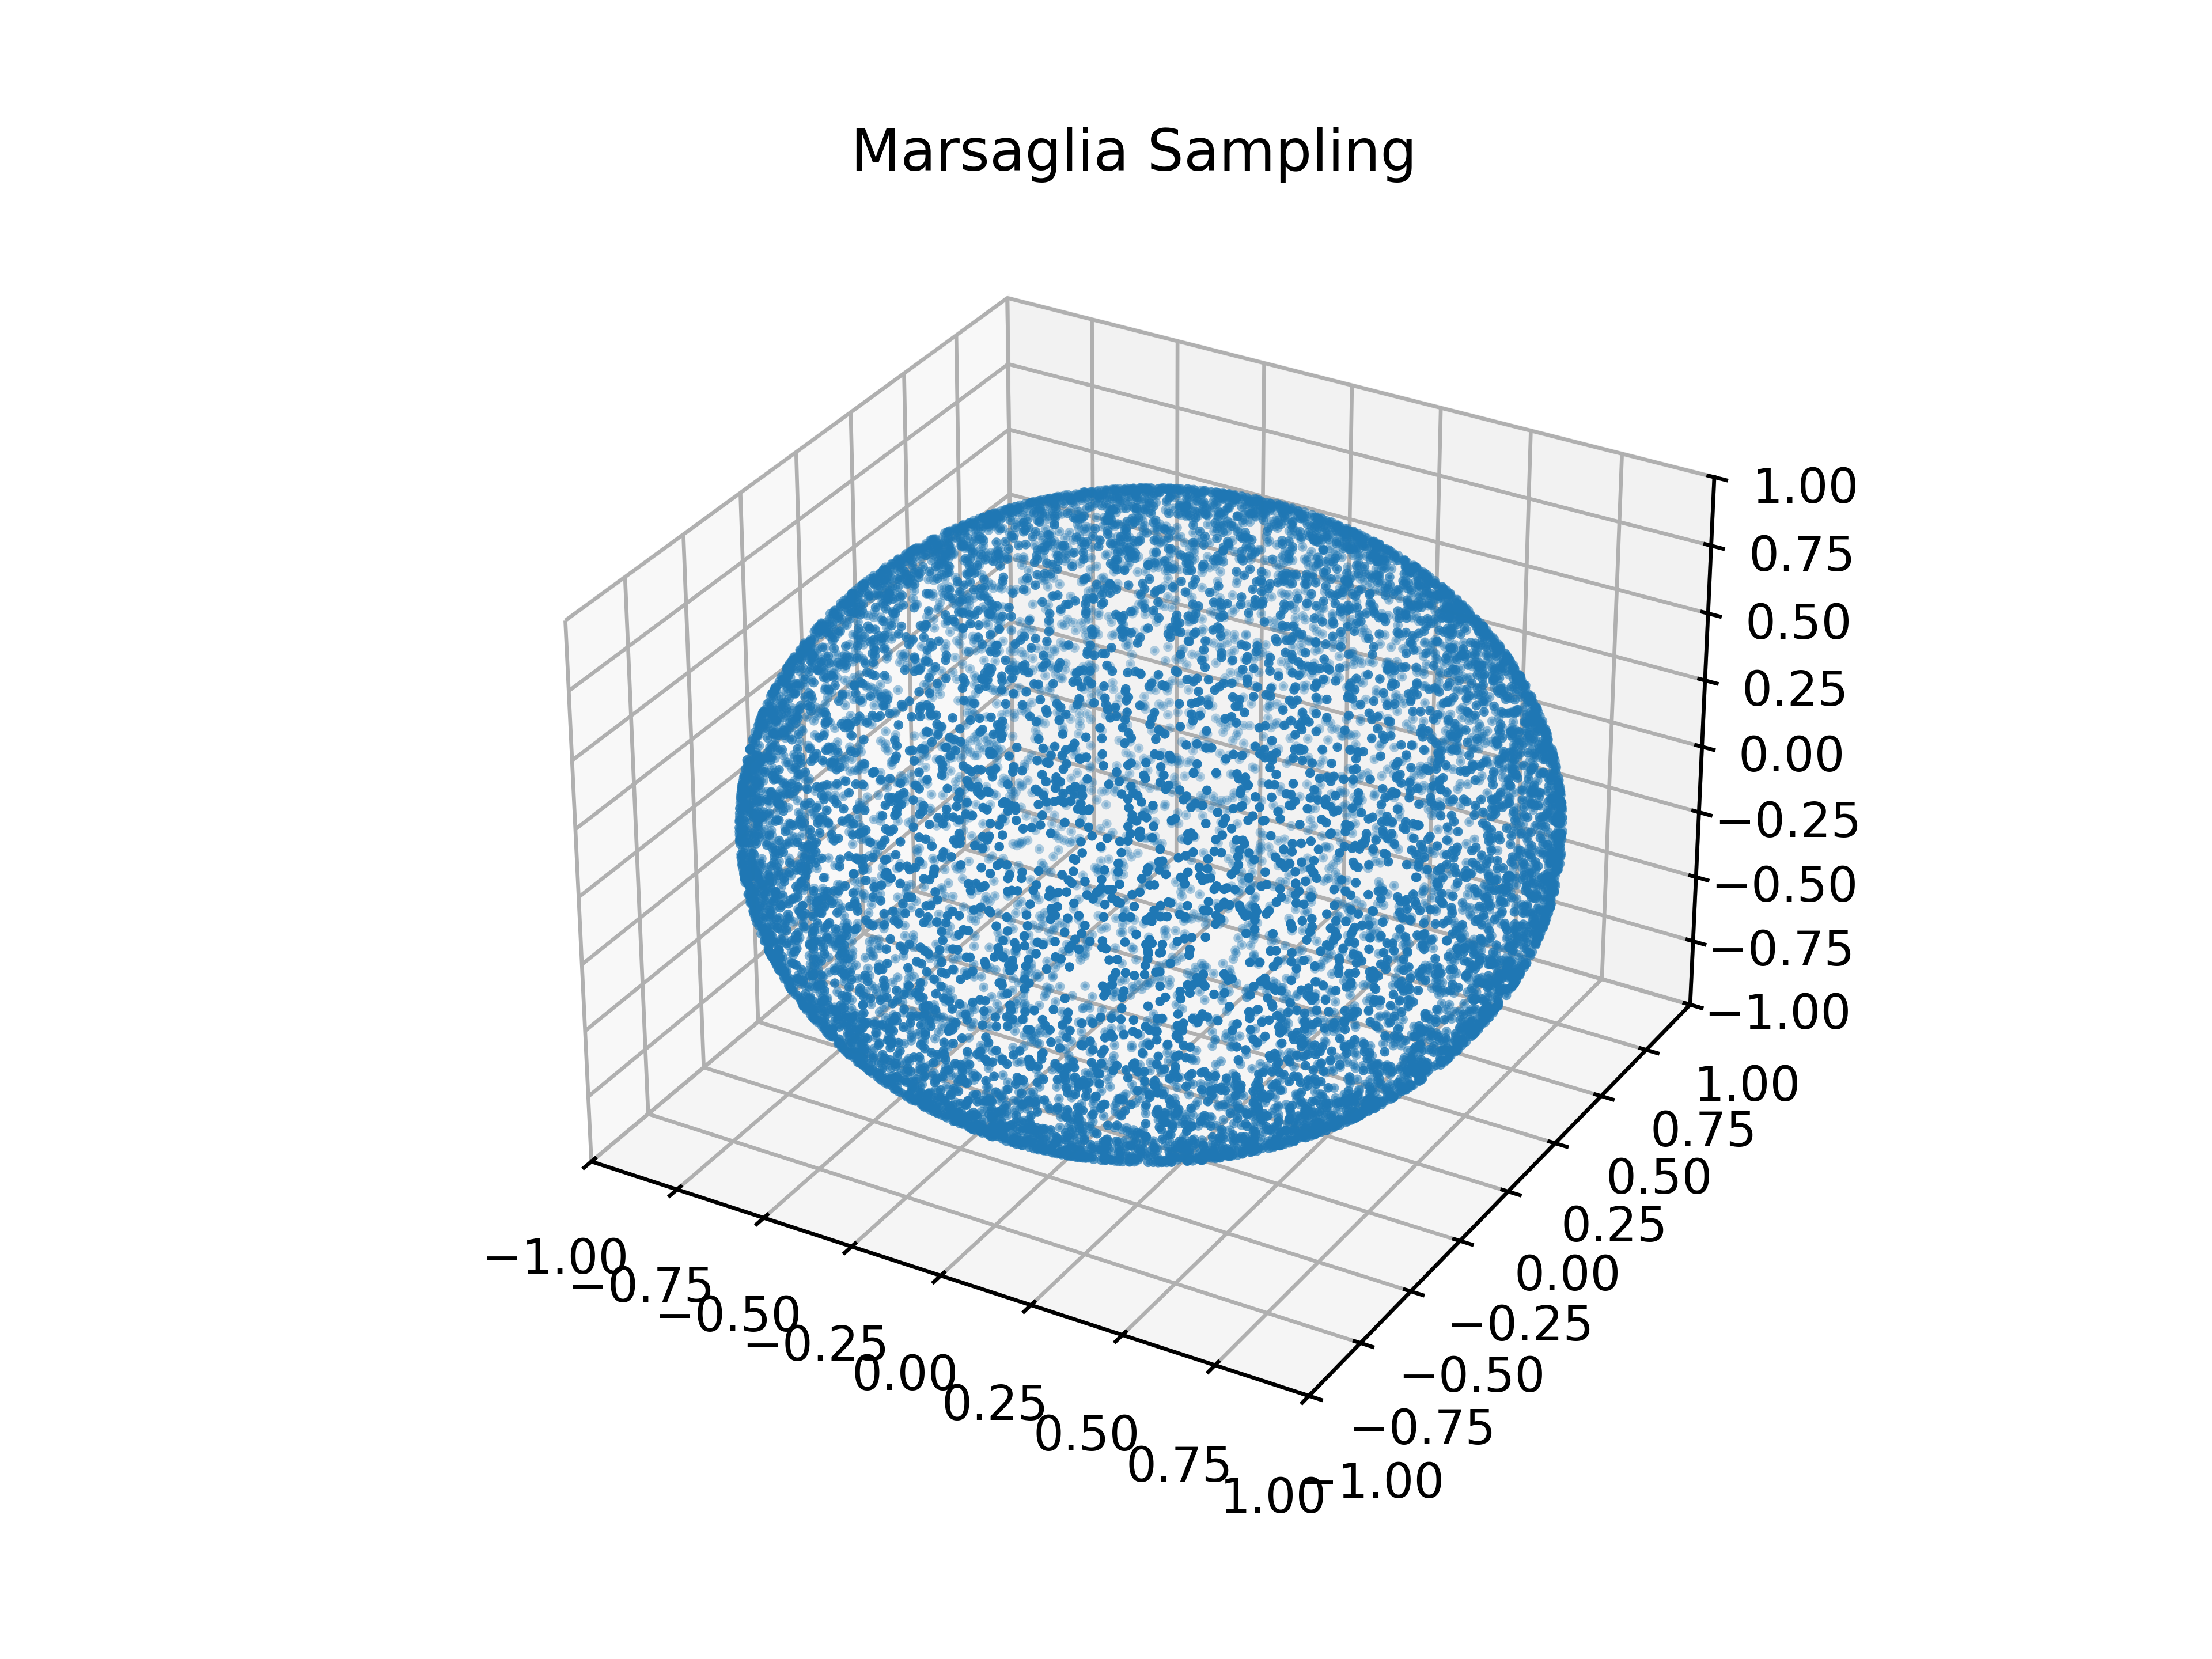
\includegraphics[width=0.6\linewidth]{photo/Marsaglia.png}
    \caption{Marsaglia算法生成的球面均匀分布}
    \label{fig:mar}
  \end{figure}

  \begin{figure}[htpb]
    \centering
    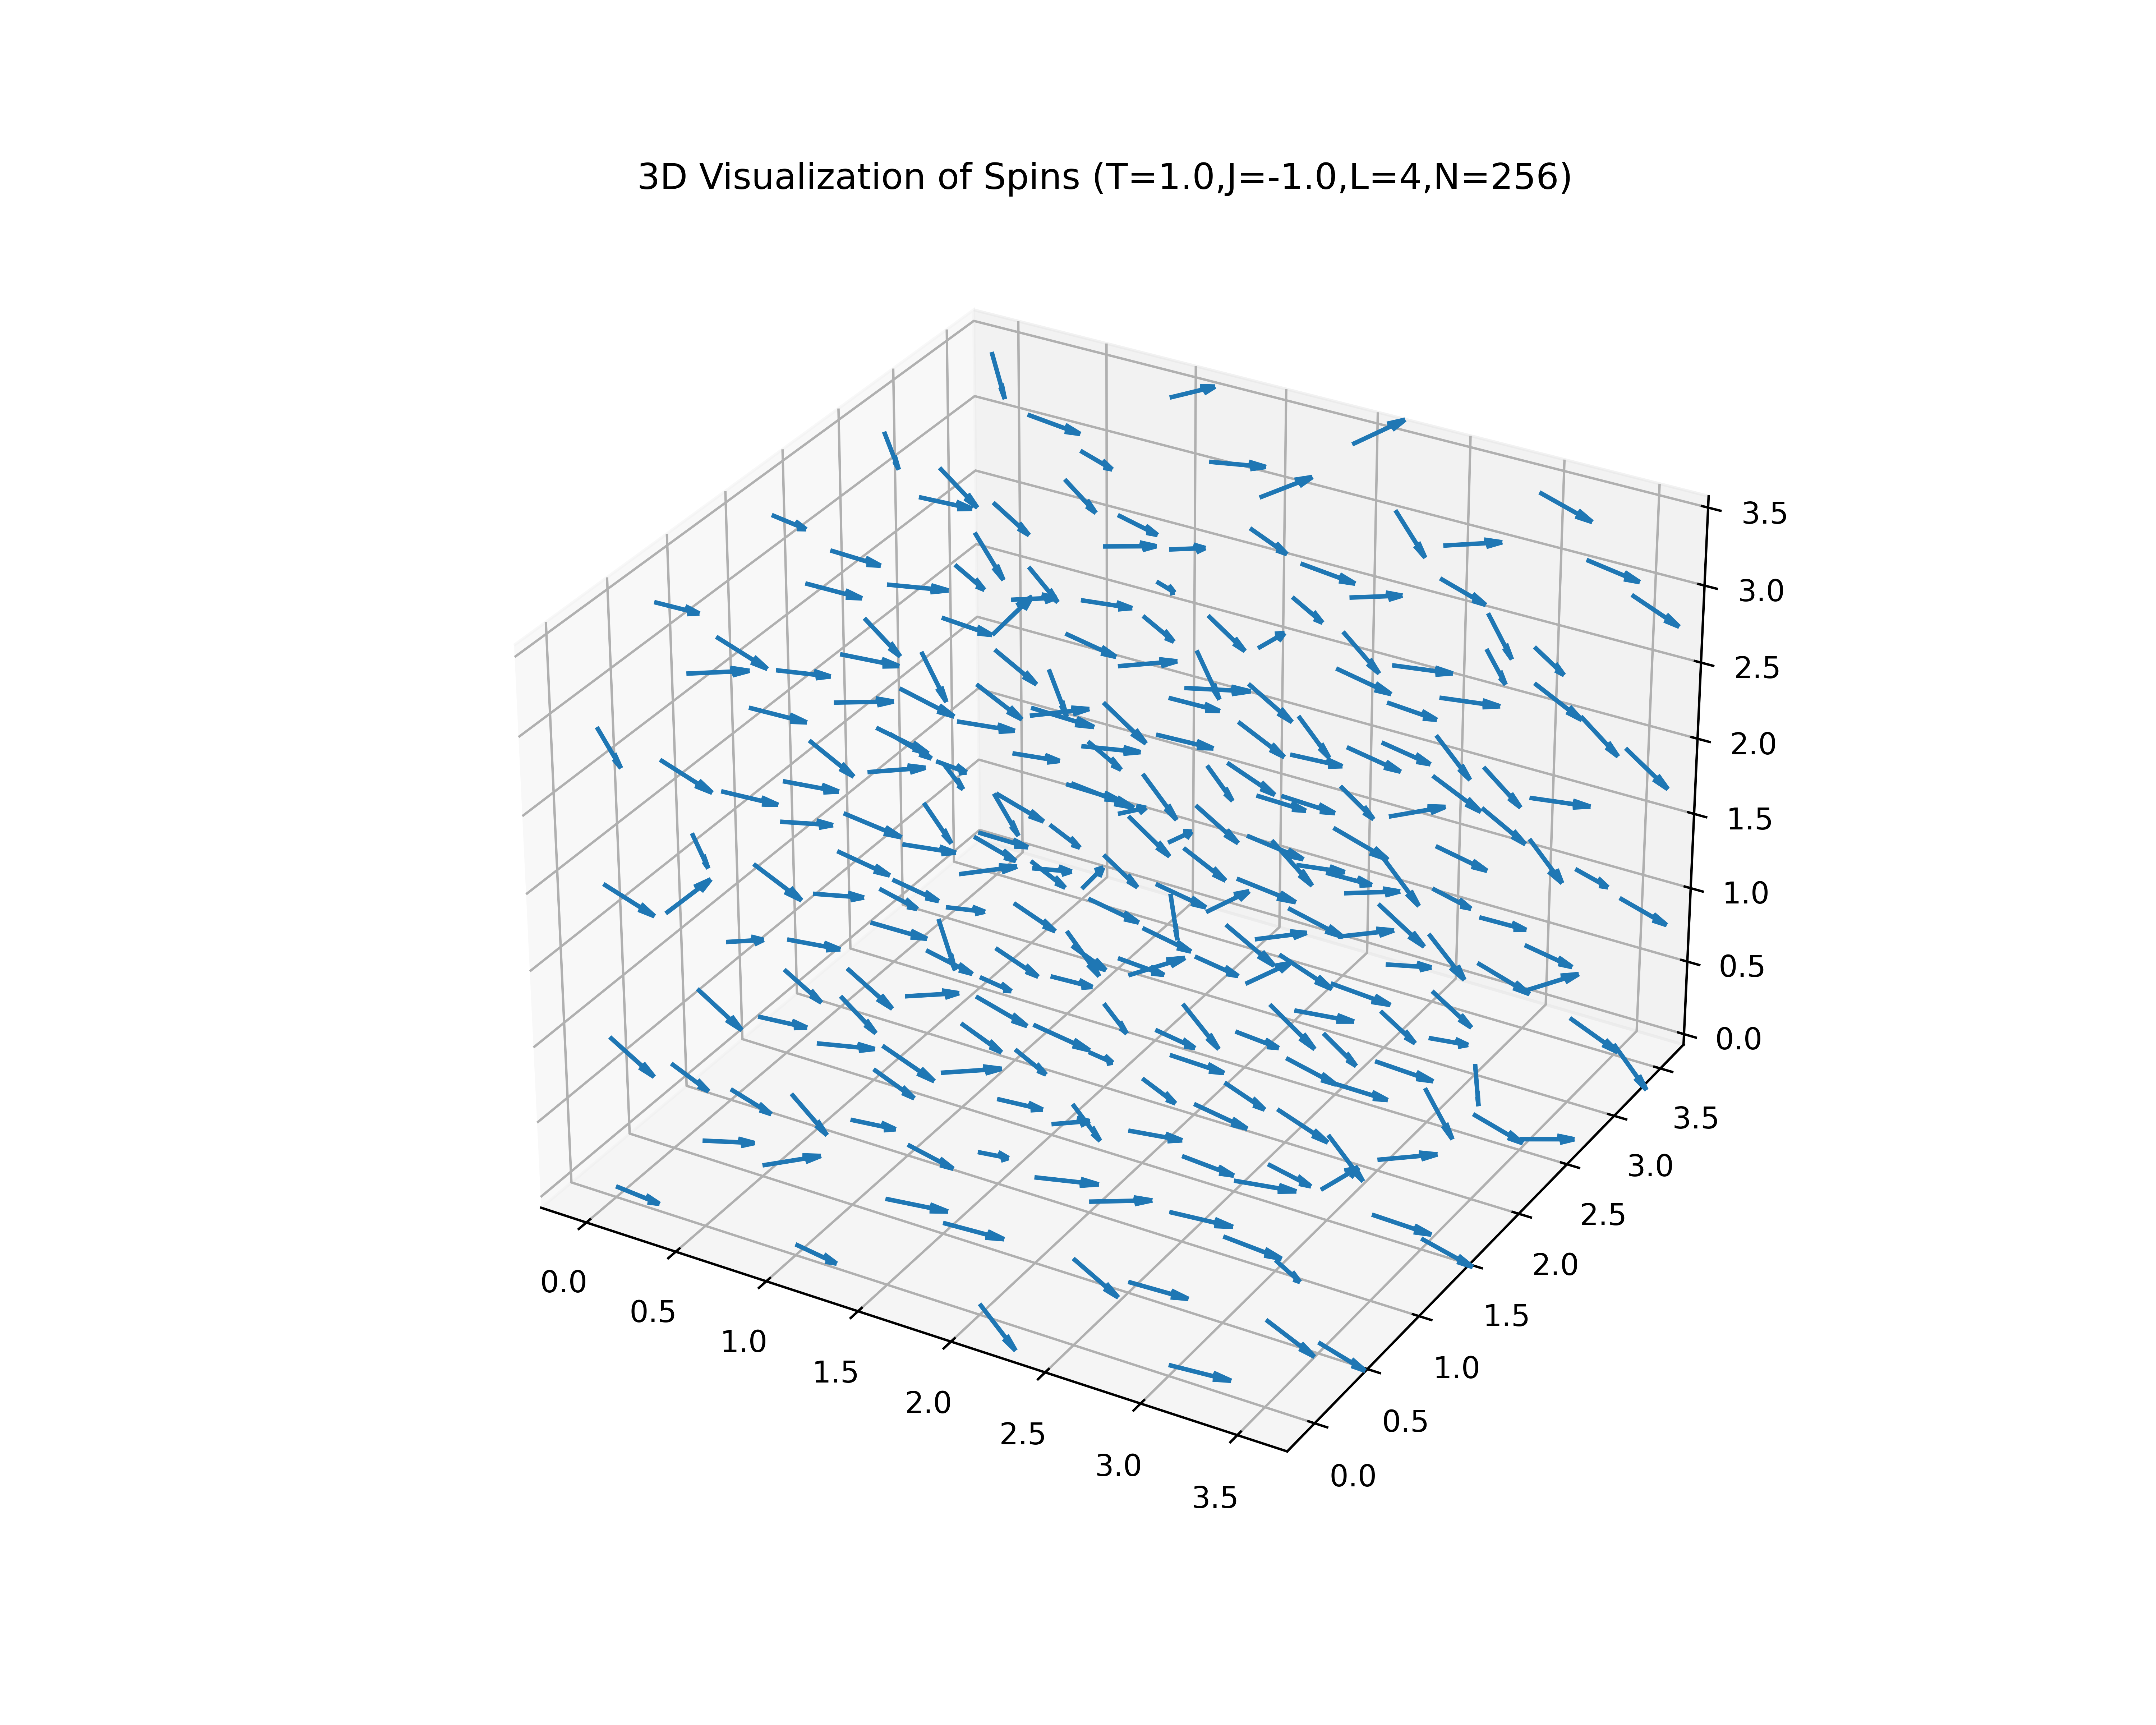
\includegraphics[width=0.6\linewidth]{photo/T=1.0.png}
    \caption{L=4,T=1.0时的平衡结构,磁矩朝向较为有序}
    \label{fig:t1}
  \end{figure}
  \begin{figure}[htpb]
    \centering
    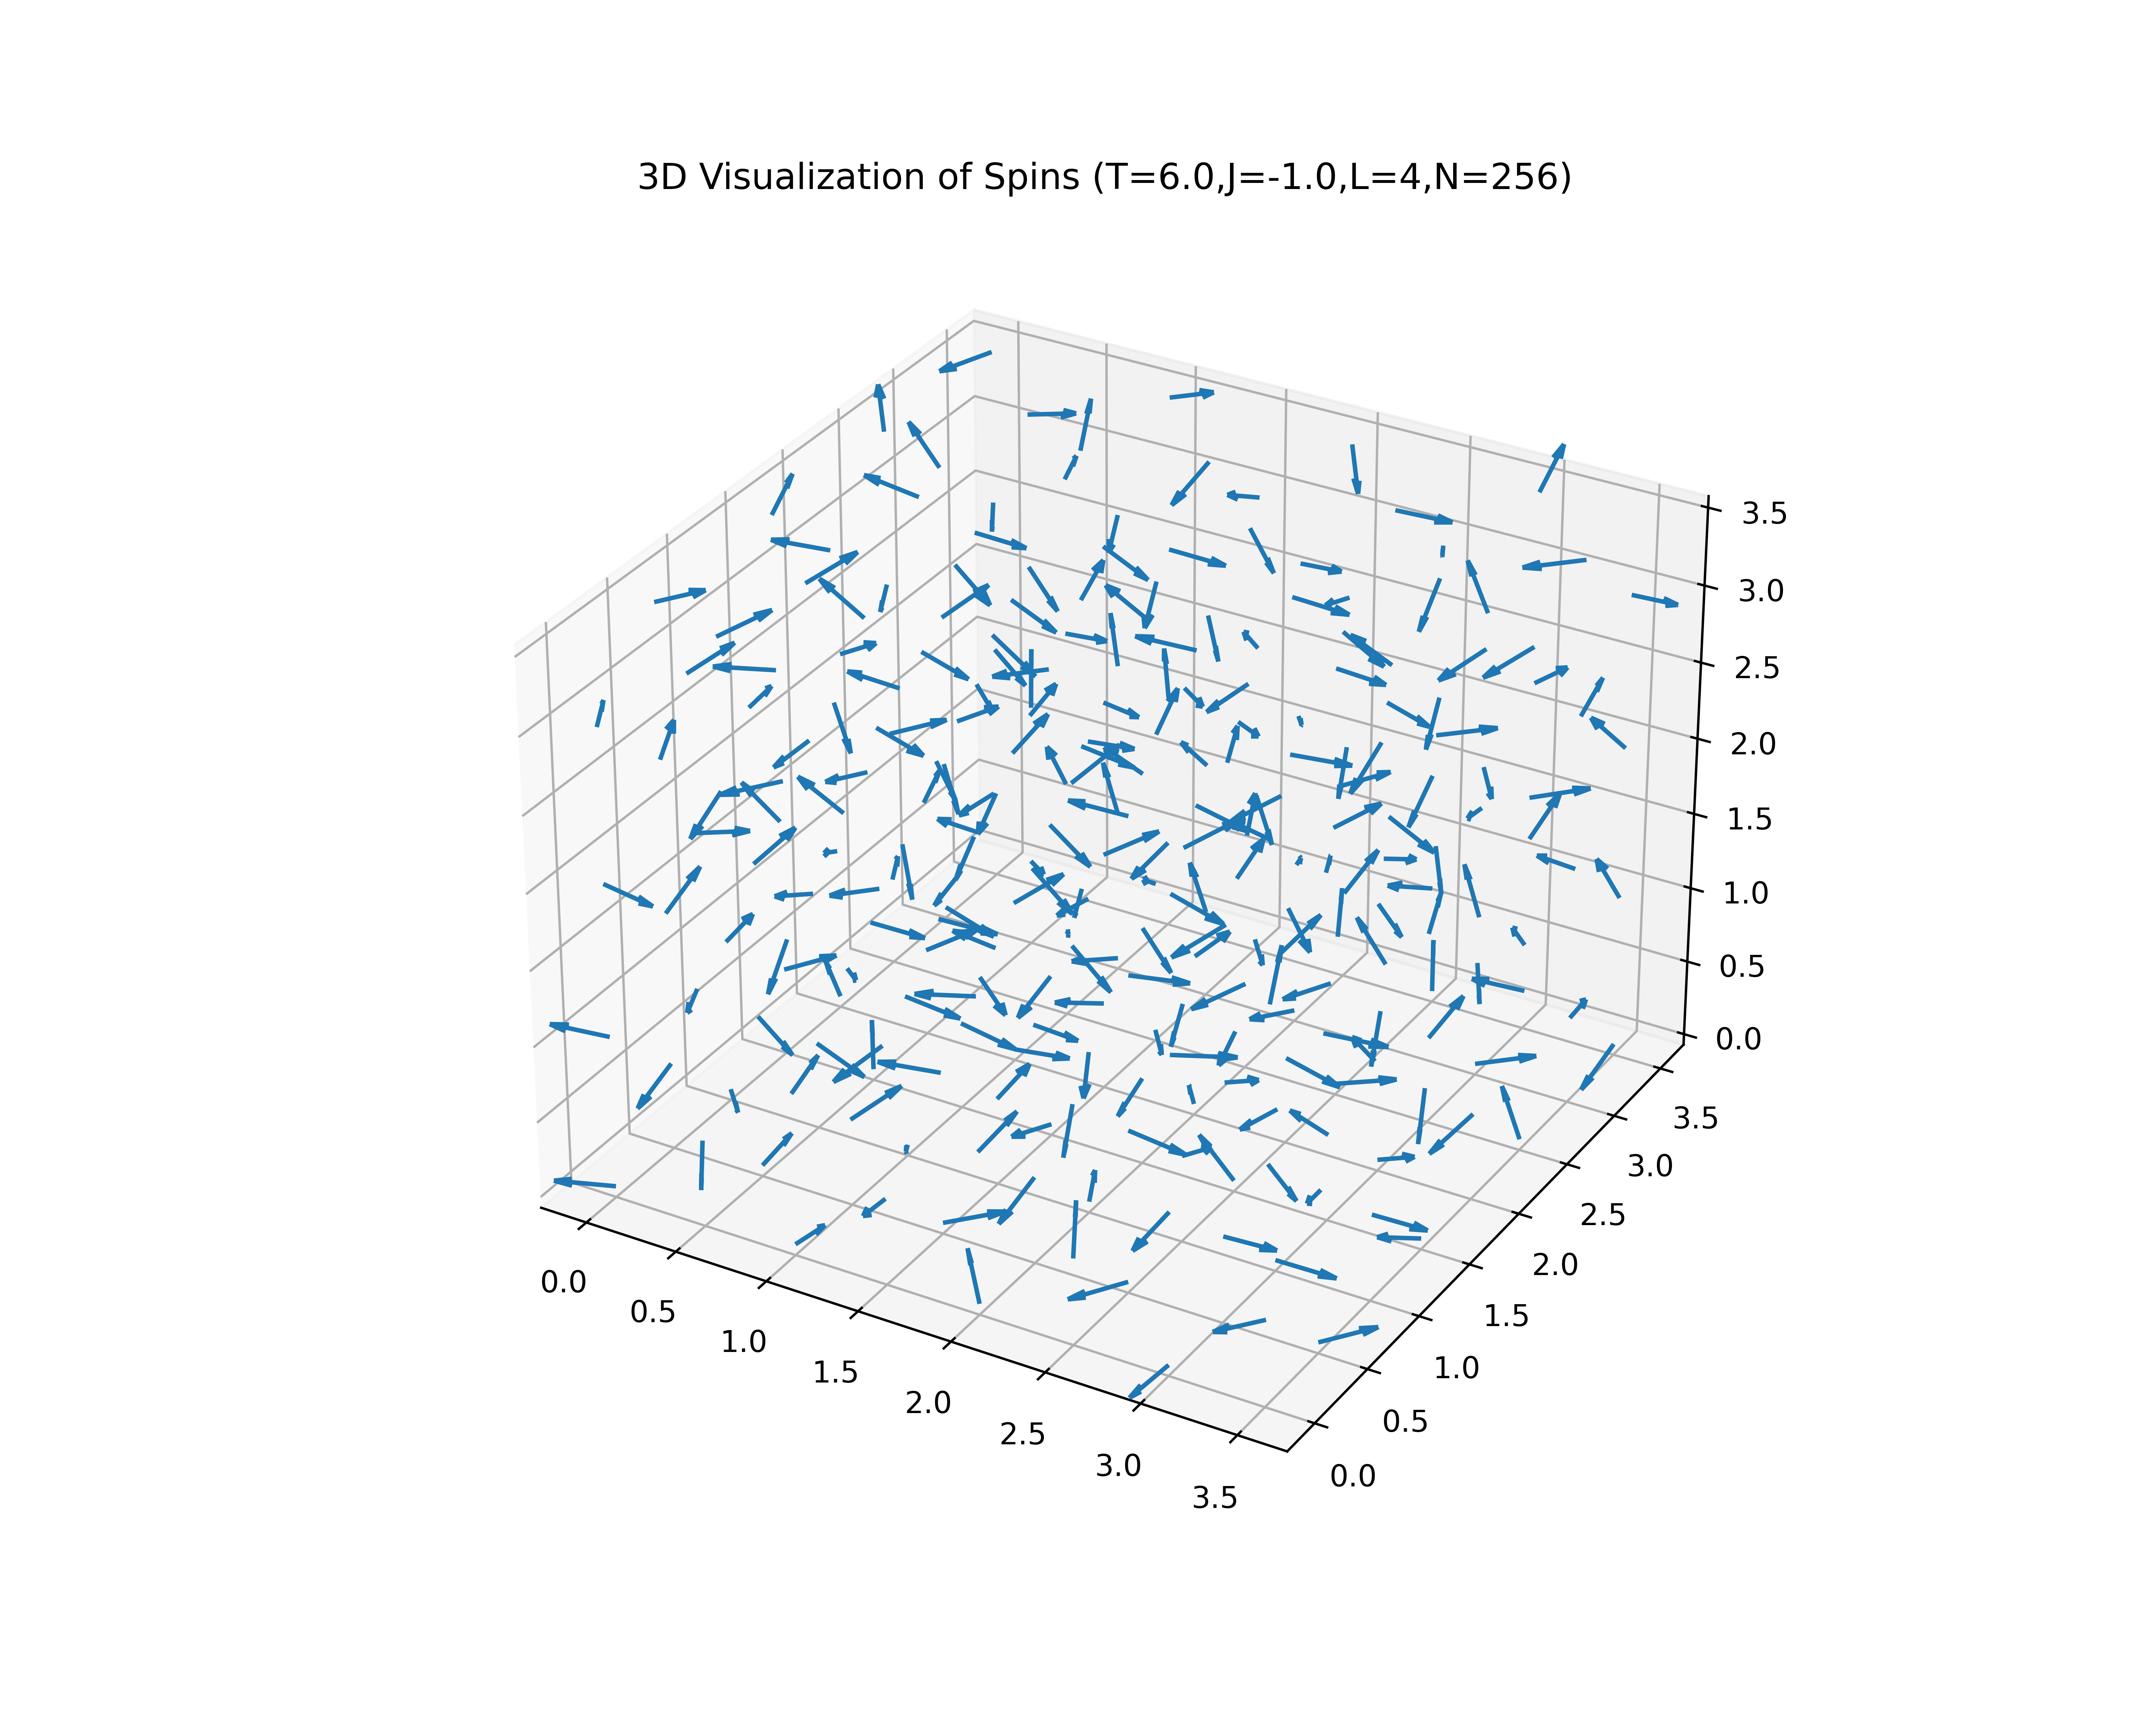
\includegraphics[width=0.6\linewidth]{photo/T=6.0.png}
    \caption{L=4,T=6.0时的平衡结构,磁矩呈混乱分布}
    \label{fig:t6}
  \end{figure}

  \begin{figure}[ht]
    \centering
    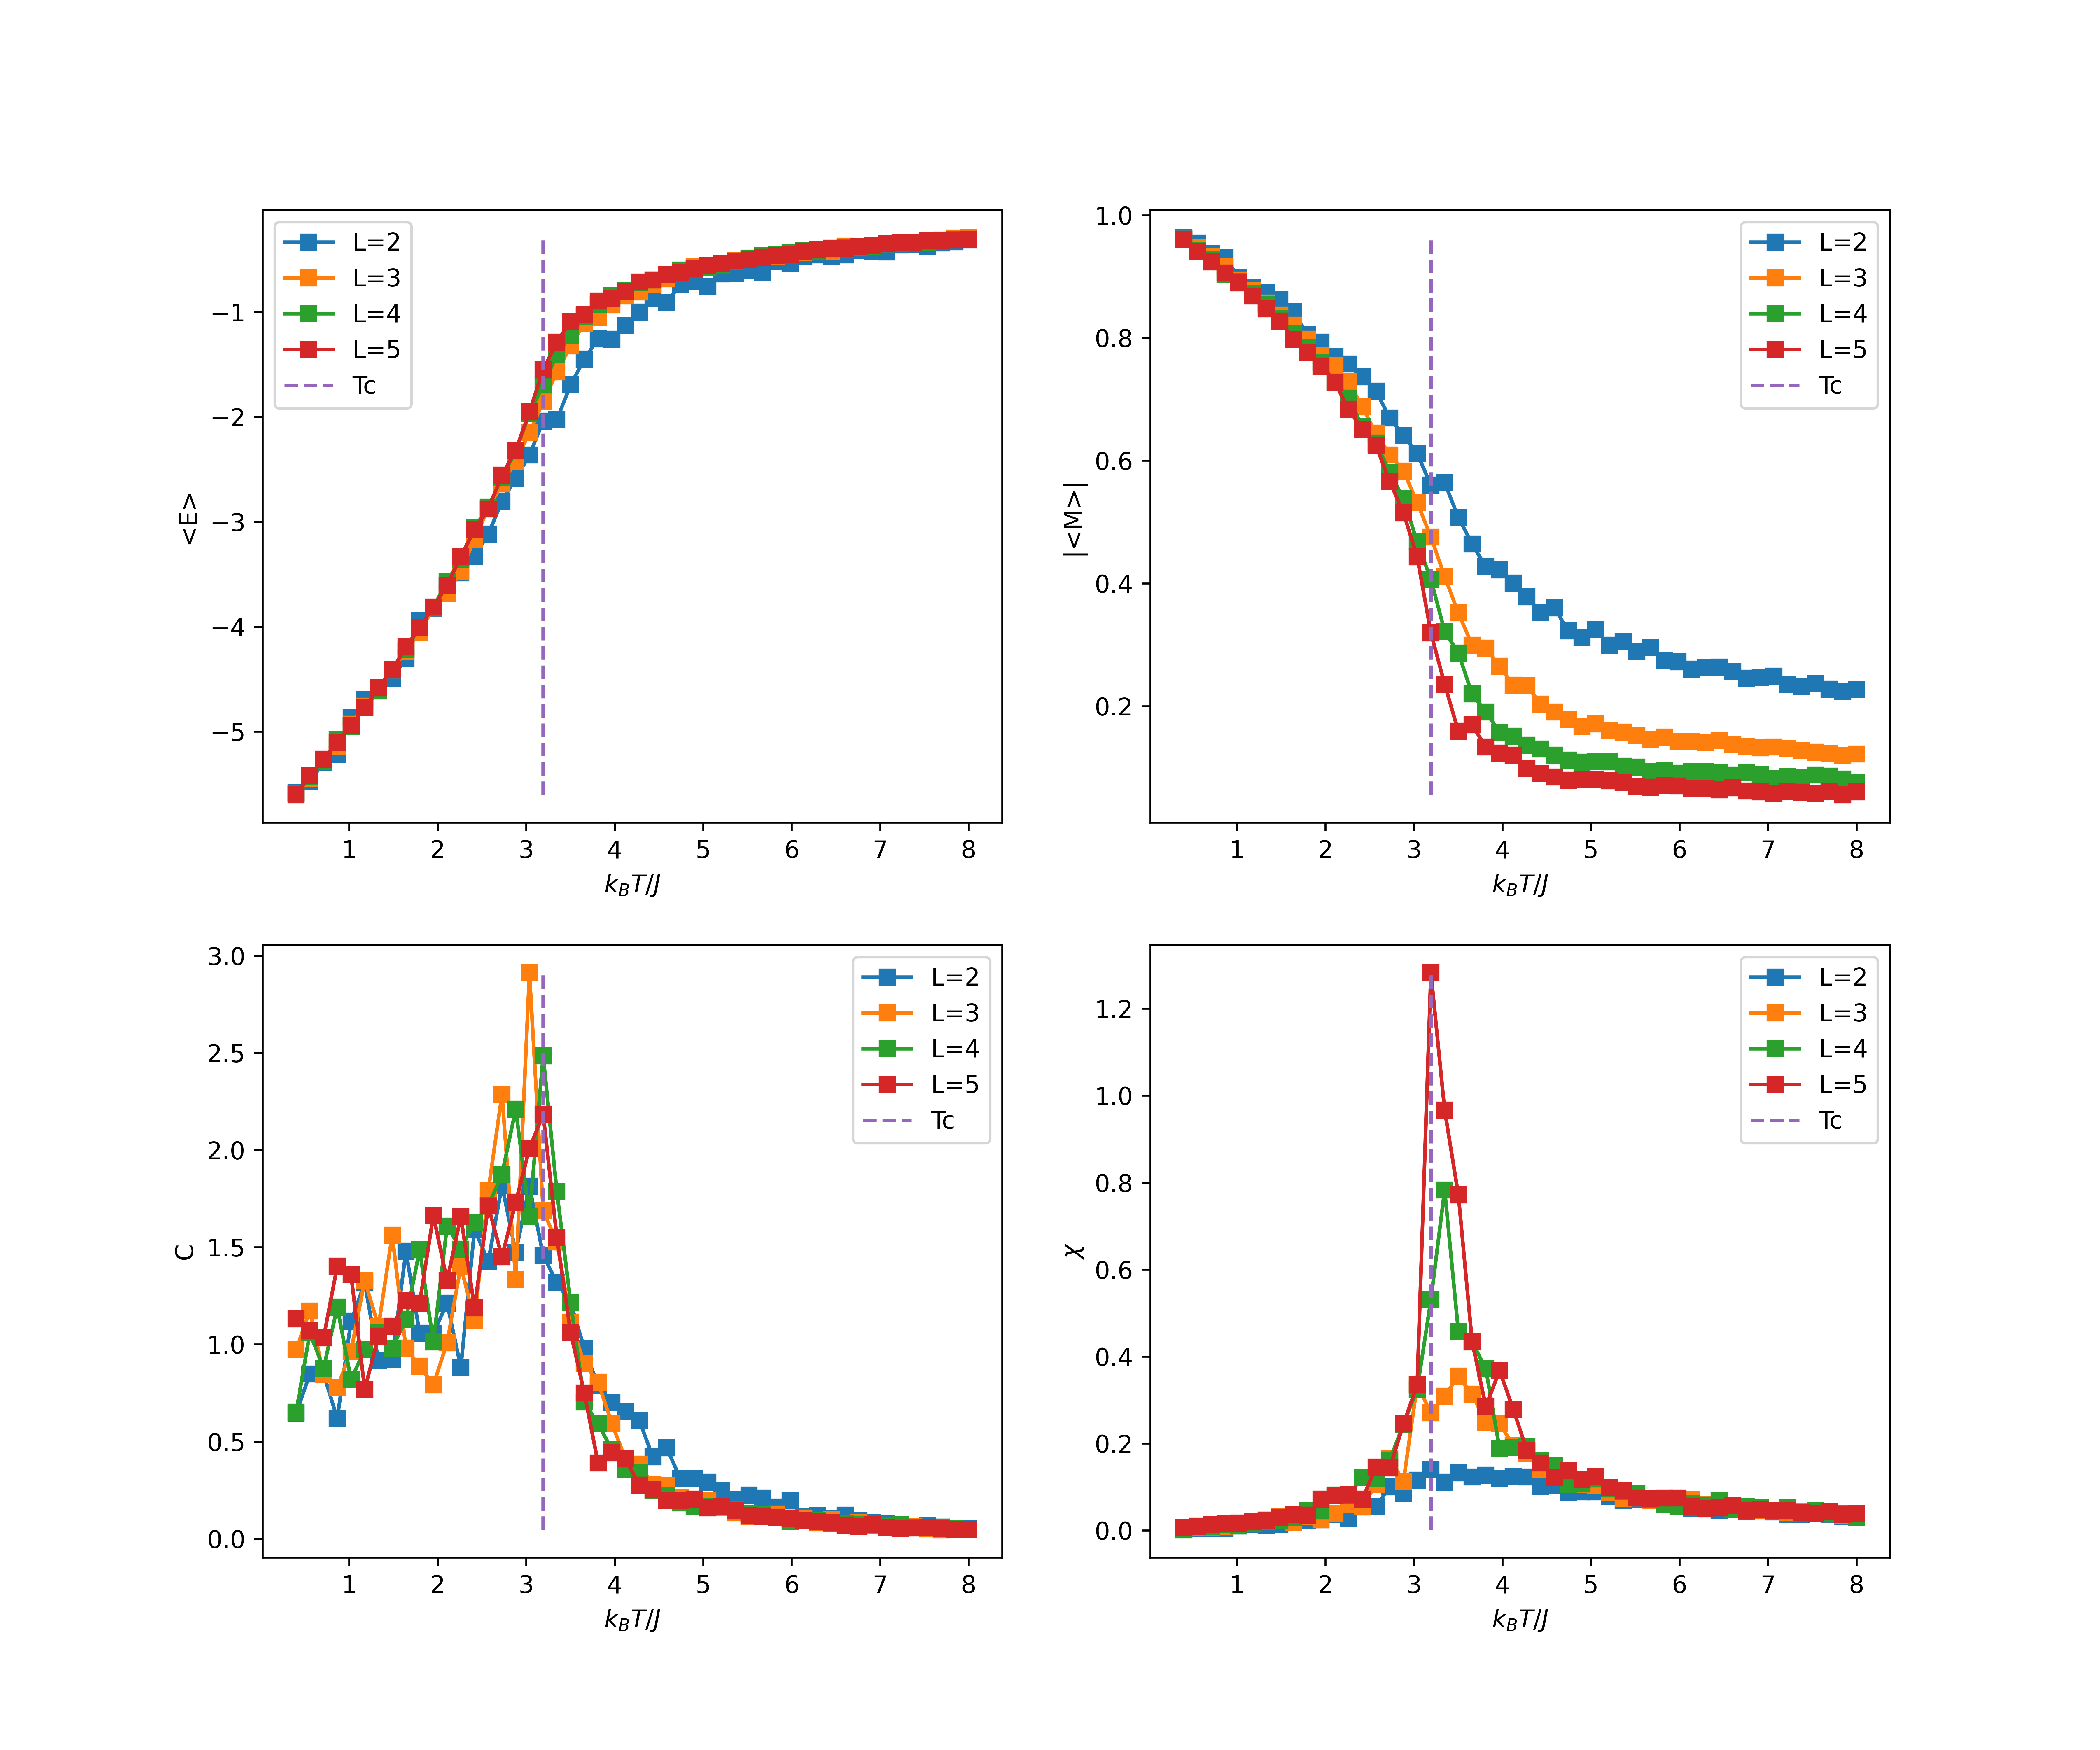
\includegraphics[width=1.0\linewidth]{photo/findTc.png}
    \caption{不同$L$,$<E>,<|M|>,C,\chi$随$T$的变化}
    \label{fig:Tc}
  \end{figure}


  \begin{figure}
    \centering
    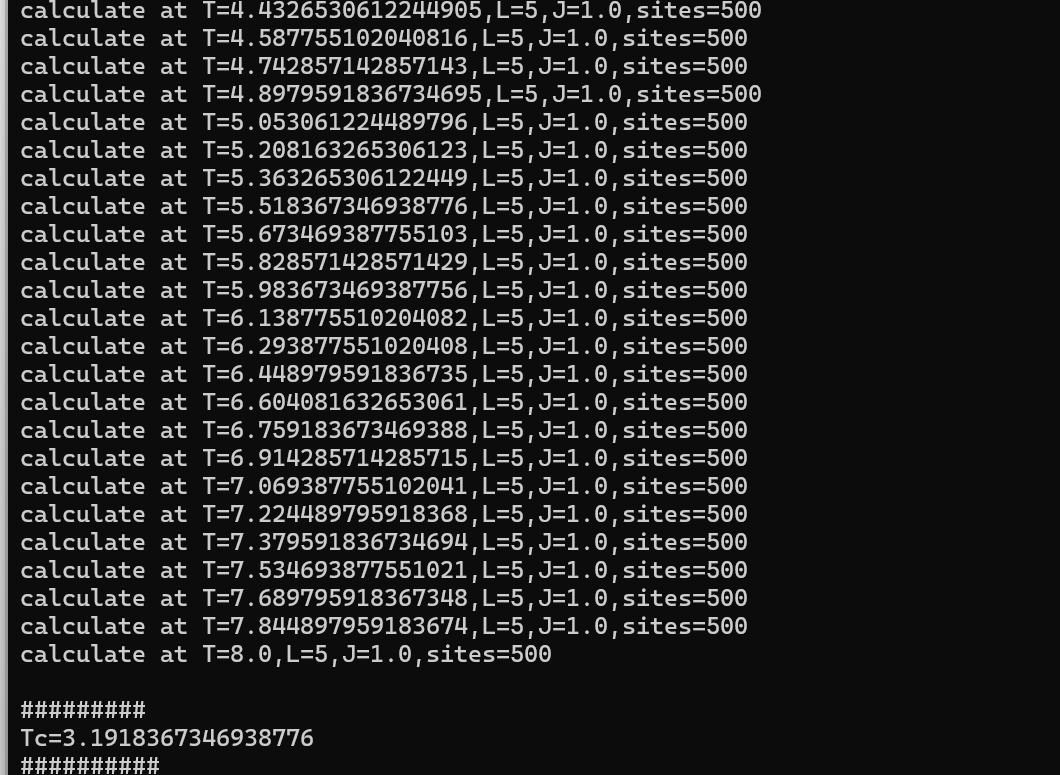
\includegraphics[width=0.6\linewidth]{photo/figp2.png}
    \caption{题目2程序运行截图}
    \label{fig:p2}
  \end{figure}

\end{document}


